% ==================== NEW PAGE FOR PROPOSAL ====================
\newpage

% Remove top margin for this page only
\vspace*{-\topmargin}
\vspace*{-\headheight}
\vspace*{-\headsep}
\vspace*{-\topskip}

% ==================== PROPOSAL HEADER WITH FULL-WIDTH BACKGROUND ====================
\noindent
\colorbox{primary}{%
    \makebox[\linewidth][c]{%
        \parbox{\paperwidth}{%
            \vspace{0.8cm}
            
            % PROPOSAL heading
            \begin{center}
                {\Huge\bfseries\color{white} PROPOSAL}
            \end{center}
            
            \vspace{0.3cm}
            
            % Divider
            \begin{center}
                \textcolor{white}{\rule{0.6\textwidth}{0.5pt}}
            \end{center}
            
            \vspace{0.3cm}
            
            % Program and Project
            \begin{center}
                {\Large\bfseries\color{white} \program{} – Summer Term}
            \end{center}
            
            \vspace{0.2cm}
            
            \begin{center}
                {\large \color{white} \projecttitle}
            \end{center}
            
            \vspace{0.4cm}
            
            % Second divider
            \begin{center}
                \textcolor{white}{\rule{0.8\textwidth}{0.3pt}}
            \end{center}
            
            \vspace{0.3cm}
            
            % Project metadata
            \begin{center}
                {\color{white}\textbf{Project:}} \projecttitle
            \end{center}
            
            \begin{center}
                {\color{white}\textbf{Mentors:}} \mentors
            \end{center}
            
            \begin{center}
                {\color{white}\textbf{Duration:}} Mid-June to end of November 2026 (part-time, 12--15 hrs/week)
            \end{center}
            
            \vspace{0.3cm}
            
            % Third divider
            \begin{center}
                \textcolor{white}{\rule{0.8\textwidth}{0.3pt}}
            \end{center}
            
            \vspace{0.3cm}
            
            % Applicant info
            \begin{center}
                {\color{white}\textbf{\myname}}
            \end{center}
            
            \begin{center}
                {\color{white}\mydegree}
            \end{center}
            
            \begin{center}
                {\color{white}\href{\githuburl}{\color{white}\mygithub}}
            \end{center}
            
            \begin{center}
                {\color{white}\mylocation}
            \end{center}
            
            \begin{center}
                {\color{white}\texttt{\myemail}}
            \end{center}
            
            \vspace{0.8cm}
        }%
    }%
}

% Restore normal spacing after the full-width box
\vspace{0.5cm}

% ==================== INDEX / TABLE OF CONTENTS ====================
\begin{center}
    {\Large\bfseries\color{primary} Index / Table of Contents}
\end{center}

\vspace{0.2cm}
\begin{center}
    \textcolor{secondary}{\rule{0.5\textwidth}{0.3pt}}
\end{center}
\vspace{0.3cm}

\tableofcontents

\newpage
\section{Executive Summary}

Hyperledger Fabric-X is not a minor release upgrade of Hyperledger Fabric. It is a different network architecture with a different operational center of gravity. In classic Fabric, Fablo can describe a network in terms of organizations, peers, orderers, certificate authorities, channels, and chaincodes, then generate a working Docker-based environment from a single \texttt{fablo-config.json}. Fabric-X changes those assumptions. The Fabric-X repository and sample deployment material show a decomposed system with separate orderer, sidecar, coordinator, verifier, validator-committer, query service, PostgreSQL, and Fabric Smart Client nodes. The bundled \texttt{xdev} sample in \texttt{fabric-x-repo/samples/tokens/compose-xdev.yml} is already enough to prove that running Fabric-X locally requires more than renaming classic Fabric containers. Its startup path depends on service-specific environment variables, routing tables, FSC node configuration, and crypto material that is currently assembled from sample scripts rather than from a tool like Fablo.

Fablo is the right foundation for solving this because it already owns the part of the developer experience that matters most: taking a compact declarative configuration and turning it into reproducible local infrastructure. The current codebase uses a Docker-based generation approach where the \texttt{setup-network} command runs inside a container to generate network artifacts using EJS templates. However, this monolithic architecture makes it difficult to support fundamentally different network types like Fabric-X without extensive modifications.

The solution was to introduce a pluggable engine architecture that separates network-type-specific logic into interchangeable engines. The implemented PoC establishes that engine framework and a Fabric-X engine that reads a single \texttt{fablo-config-fabricx.json}, validates it against a versioned JSON schema, generates the required bootstrap artifacts, and brings up a working local Fabric-X network. The engine architecture maintains backward compatibility with classic Fabric while enabling clean extension for new network types.

\begin{tcolorbox}[colback=blue!5!white, colframe=blue!60!black,
  title=Core Deliverable, fonttitle=\bfseries, arc=4pt]
A pluggable engine architecture for Fablo with a production-quality Fabric-X engine that reads a single \texttt{fablo-config-fabricx.json}, validates it against a versioned JSON schema, generates all Docker Compose and configuration artifacts, and bootstraps a working local Fabric-X network with a single command --- with full lifecycle management (\texttt{fablo up}, \texttt{fablo down}, \texttt{fablo status}, \texttt{fablo reset}), automated e2e tests mirroring Fablo's existing test structure, and contributor documentation.

The implementation is now fully working and has been verified end-to-end, leveraging the pluggable engine architecture. Mentor feedback confirmed that separating `$schema` is the correct design approach, as Fabric-X fundamentally differs from classic Fabric in its schema requirements. The following commands have been verified: \texttt{fablo init --fabricx}, \texttt{fablo generate fablo-config-fabricx.json fablo-target/fabricx}, \texttt{fablo up fablo-config-fabricx.json fablo-target/fabricx}, \texttt{fablo status fablo-config-fabricx.json fablo-target/fabricx}, and \texttt{fablo down fablo-config-fabricx.json fablo-target/fabricx}.
\end{tcolorbox}

\begin{tcolorbox}[colback=blue!5!white, colframe=blue!60!black,
  title=Stretch Goals --- conditional on core completion by Week 24,
  fonttitle=\bfseries, arc=4pt]
\begin{itemize}[leftmargin=*]
  \item Multi-org Fabric-X topology support
  \item Separate-container committer, validator, verifier, coordinator, and orderer deployment
  \item CI integration example for Fabric-X networks
  \item Fablo UI support for Fabric-X configs and topology visualization
\end{itemize}
\end{tcolorbox}

\section{The Problem: Why This Work Matters}

I see the main problem as a developer-experience gap. Fabric-X is promising, but the local workflow is still too fragmented for fast experimentation. A contributor who wants to try it locally has to understand a decomposed service model, generate bootstrap artifacts, start multiple interdependent components in the right order, and run post-start configuration steps before the network is actually useful.

That makes Fabric-X harder to approach than it needs to be. It slows onboarding, makes demos harder to prepare, and turns simple experimentation into environment work. For a project that is still evolving, that friction matters: if the first local experience is complicated, fewer people will try it and fewer contributors will build confidence working on it.


\subsection{What Fablo does today and why it is the right foundation}

I chose Fablo as the foundation because it already solves the right problem for classic Fabric: it turns a compact declarative config into a runnable local environment and gives the user a clean lifecycle around it. That is exactly the user experience Fabric-X is missing today.

For this project, I do not need to invent a new CLI model from scratch. I can build on an existing tool that already knows how to generate artifacts, manage target directories, and present a simple local workflow. That lets me focus on the real challenge: representing Fabric-X correctly while preserving the simplicity that makes Fablo useful.

\subsection{Why the integration is non-trivial}

The integration is non-trivial because Fabric-X is not just another Fabric version. It changes the runtime model. Instead of a small number of familiar components, I have to deal with a decomposed orderer, a decomposed committer stack, more service-to-service wiring, more ports, a more delicate bootstrap sequence, and an additional configuration step after startup.

That means I cannot treat Fabric-X support as a thin template variation on the classic path. I need a structure that lets me isolate Fabric-X behavior, keep classic Fabric stable, and still grow from a simple local bootstrap into a fuller implementation over time. That is why the architecture choice is central to this project rather than just an implementation detail.

\section{Technical Background and Research}

\subsection{Initial questions}

\begin{table}[h]
\centering
\begin{tabularx}{\textwidth}{|p{2.6cm}|X|X|p{1.6cm}|}
\hline
\textbf{Approach} & \textbf{Advantages} & \textbf{Disadvantages} & \textbf{Verdict} \\
\hline
Separate repository & Total isolation from classic Fabric code; freedom to tailor commands, schemas, and templates only for Fabric-X; lower short-term coupling to historic Fablo assumptions. & Duplicates Fablo's CLI contract, target-directory handling, config parsing, docs surface, and test style; splits the contributor community; turns Fabric-X support into a parallel tool instead of an extension of the standard Fabric bootstrap workflow. & Rejected \\
\hline
Wrapper over Ansible & Fastest route to a demo if the only goal is to invoke existing sample tooling; preserves upstream sample scripts without deep integration work. & Leaves the developer with a two-layer mental model; errors surface through wrapper indirection; does not resolve schema mismatch; keeps ownership of generated artifacts outside Fablo; fails to create a real pluggable architecture. & Rejected \\
\hline
Pluggable engine in Fablo & Reuses mature commands, test patterns, target-dir logic, and documentation expectations; keeps classic behavior intact; isolates Fabric-X logic under \texttt{src/engines/fabricx/}; allows a future third engine without changing core CLI commands. & Requires careful architectural planning; needs careful handling of the existing Docker-based generation approach. & \textbf{Selected} \\
\hline
\end{tabularx}
\caption{Integration approach evaluation}
\label{tab:approaches}
\end{table}

The pluggable engine is the correct architectural choice because it enables clean support for different network types while maintaining Fablo's established user experience. The current Docker-based generation approach works for classic Fabric but cannot easily accommodate Fabric-X's different topology and configuration requirements. By introducing a pluggable engine architecture, we can isolate network-type-specific logic while preserving the existing CLI interface and generation workflow.

I selected the pluggable engine approach because it gives me a clean seam for Fabric-X without forcing classic Fabric and Fabric-X to share an artificial schema or a fragile set of conditional branches. It also keeps open the possibility of a third engine later, which is important if the architecture is meant to be a real extension point rather than a one-off exception.

\subsection{Initial research: Fablo codebase}
\begin{figure}[h]
\centering
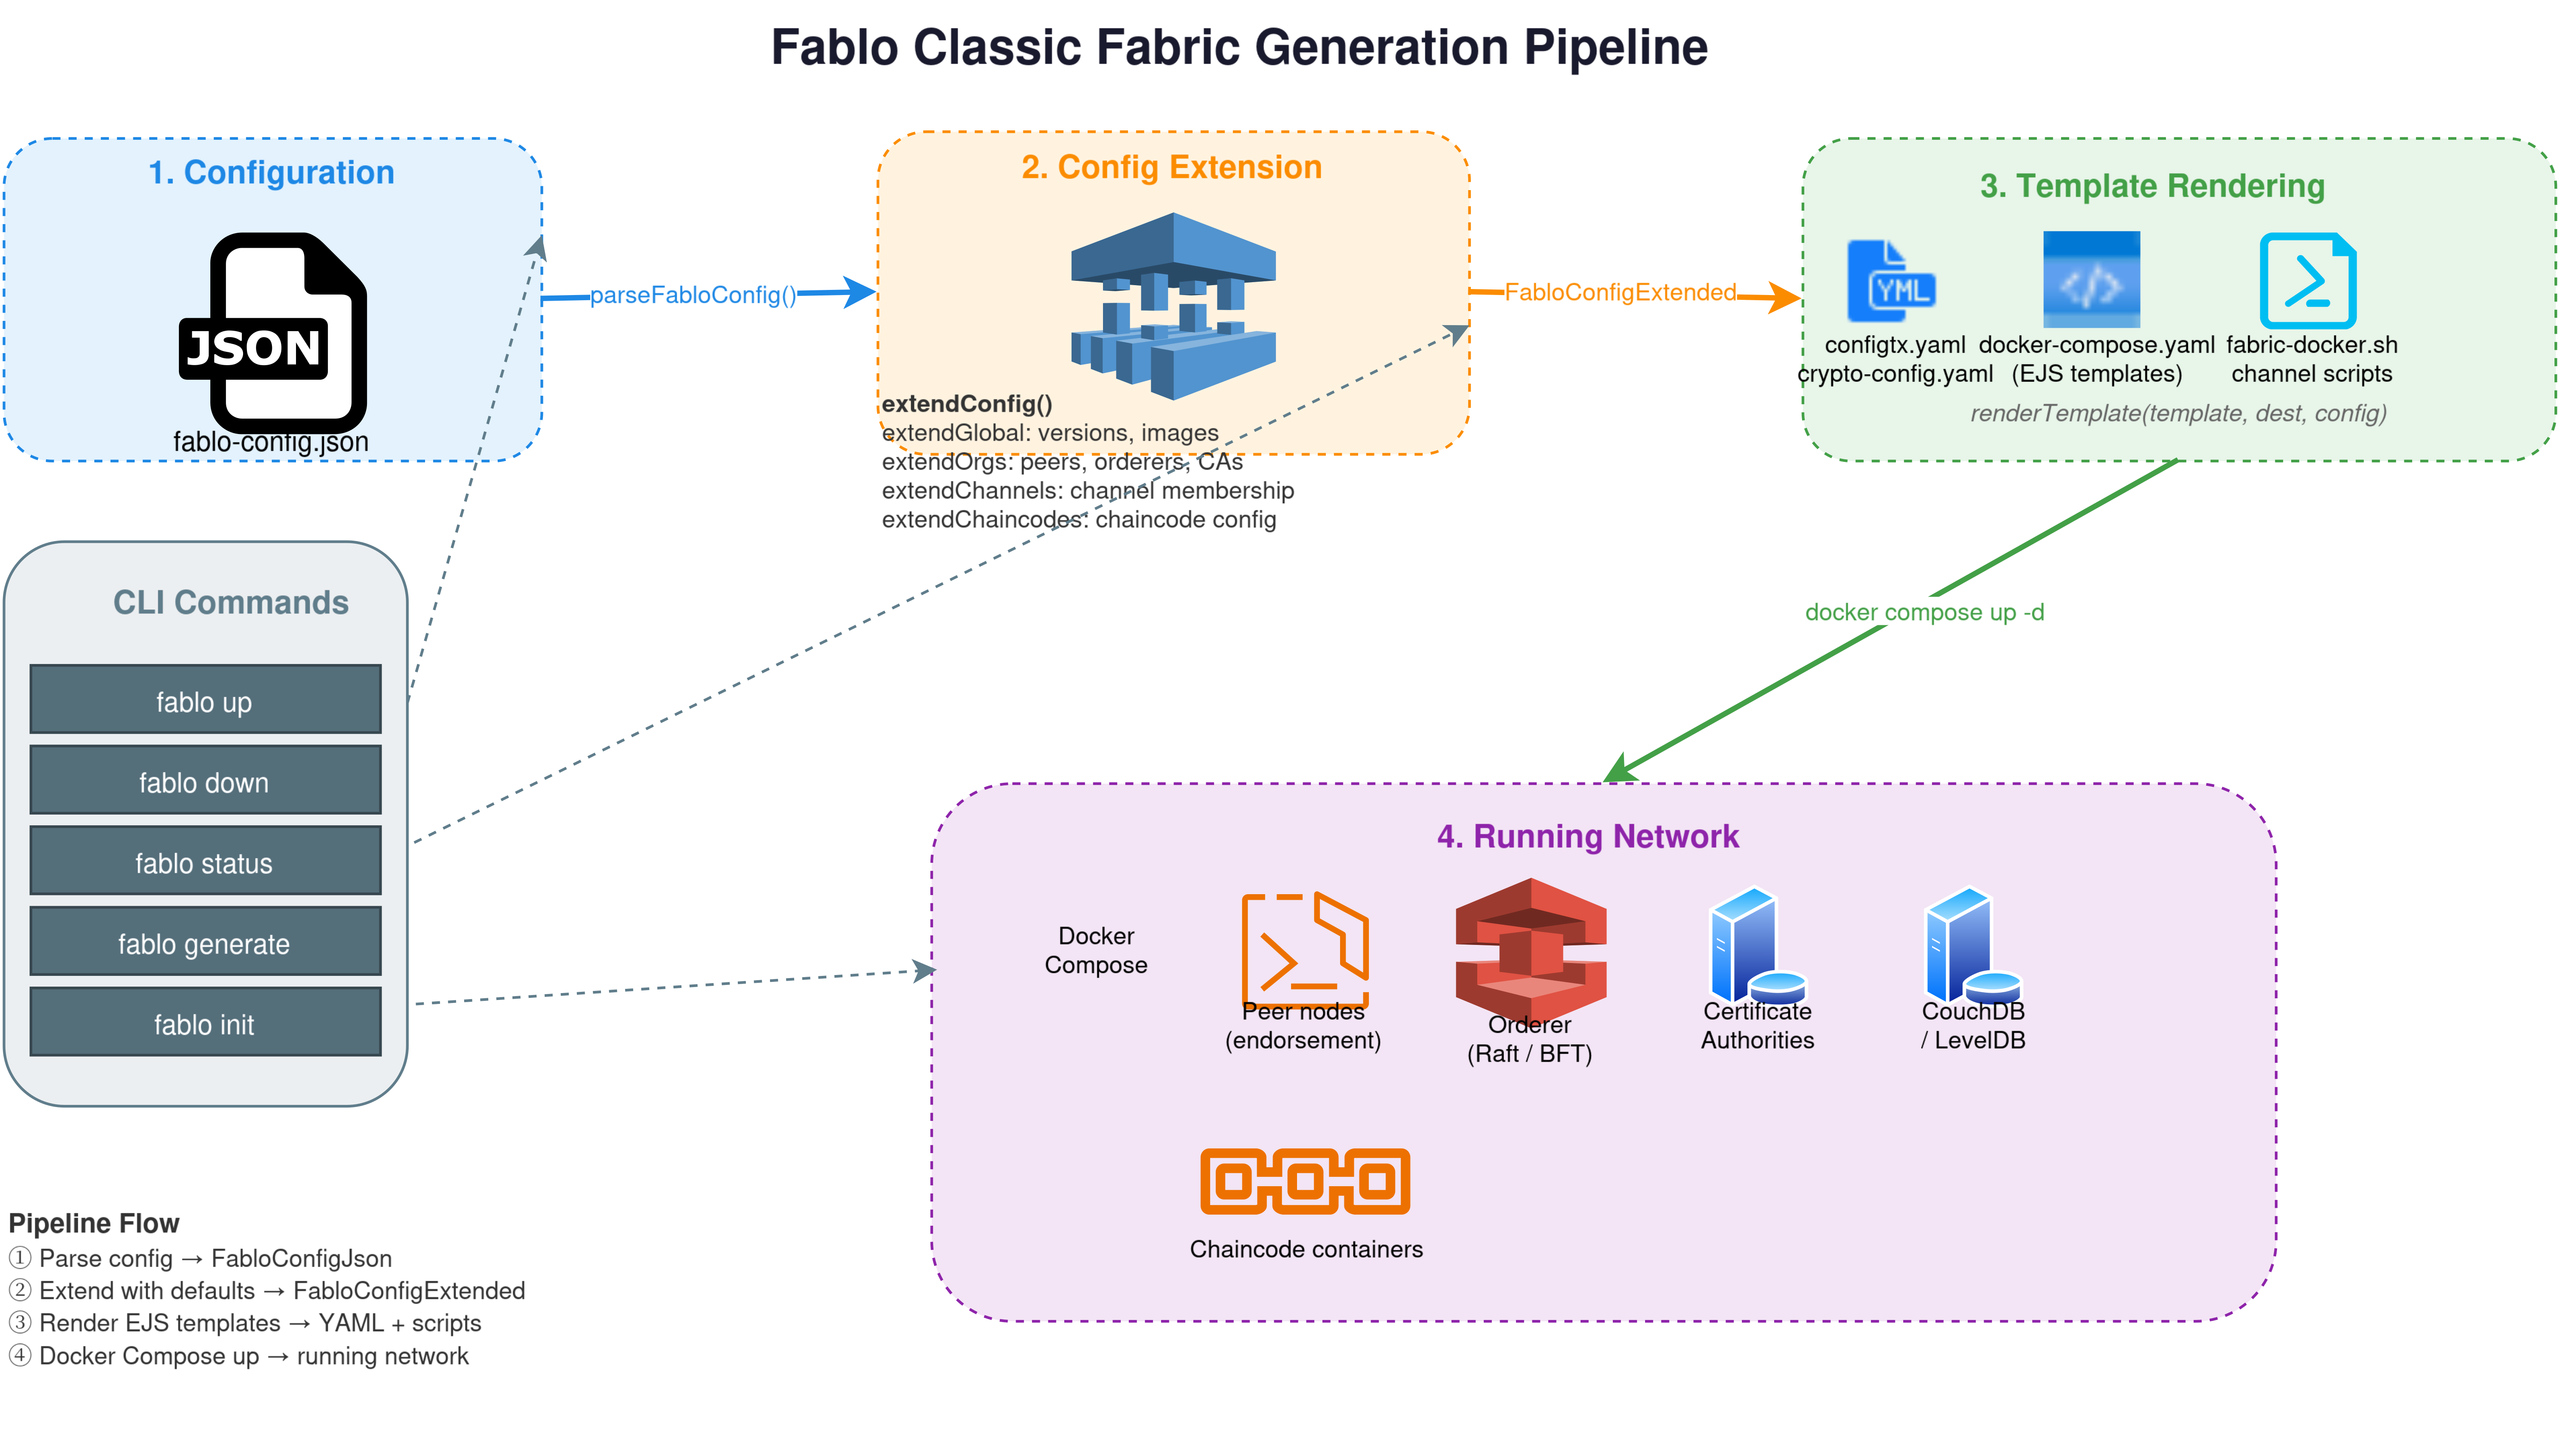
\includegraphics[width=\textwidth]{fablo_originalarchitecture_diagram.png}
\caption{Classic Fablo generation pipeline}
\label{fig:fablo-classic-pipeline}
\end{figure}

\begin{table}[h]
\centering
\begin{tabularx}{\textwidth}{|l|X|}
\hline
\textbf{Layer} & \textbf{Finding from source reading} \\
\hline
Config schema & Classic configs use \texttt{\$schema}, \texttt{global}, \texttt{orgs}, \texttt{channels}, \texttt{chaincodes}, and \texttt{hooks} as defined in \texttt{src/types/FabloConfigJson.ts}. \\
\hline
Generation pipeline & Now uses a pluggable engine architecture. For classic Fabric, it delegates to the existing Docker-based generation via \texttt{ClassicFabricEngine}. For Fabric-X, \texttt{FabricXEngine} generates artifacts directly. \\
\hline
Command structure & Oclif-based CLI. Core commands (\texttt{generate}, \texttt{up}, \texttt{down}, \texttt{status}) are engine-agnostic and delegate to the appropriate \texttt{FabloEngine} implementation. \\
\hline
Template system & Uses EJS templates in \texttt{src/setup-docker/templates/} for generating Docker Compose files, connection profiles, CA configs, and utility scripts. \\
\hline
E2E test pattern & \texttt{e2e-network/docker/test-01-v3-simple.sh} builds, initializes, runs, waits for logs, performs functional checks, exercises lifecycle commands, and tears down. \\
\hline
Type system & \texttt{src/types/FabloConfigJson.ts} defines the configuration structure with proper TypeScript interfaces. \\
\hline
\end{tabularx}
\caption{Current Fablo codebase --- confirmed architecture from source reading}
\label{tab:fablo-analysis}
\end{table}

\subsection{Initial research: Fabric-X architecture}

My implemented PoC deliberately targets the bundled \texttt{xdev} topology because that is the smallest viable integration surface that still represents real Fabric-X behavior. In that bundled local model, database, orderer, and committer behavior are started together inside one test-node flow. This table, however, describes the individual decomposed components that make up the full Fabric-X architecture. That smaller bundled path is enough to prove engine architecture, lifecycle delegation, template rendering, default port handling, and schema-first detection without taking on the full burden of a decomposed multi-service topology on day one.

\begin{table}[h]
\centering
\begin{tabularx}{\textwidth}{|l|X|}
\hline
\textbf{Component} & \textbf{Role and config surface} \\
\hline
Arma Orderer & The orderer stack is decomposed into routers, batchers, consenters, and assemblers. In realistic local layouts, each role has its own RPC and metrics ports rather than sharing one orderer endpoint. \\
\hline
Endorser & In the current PoC schema, endorser is an FSC node role. It receives a generated \texttt{core.yaml} with node identity, P2P endpoint, routing references, Fabric-X driver settings, and token namespace wiring. \\
\hline
Validator-Committer & The validator-committer is its own committer component. It represents the validation and commitment half of the decomposed commit path. \\
\hline
Sidecar & The sidecar is the Fabric-facing entry point for FSC nodes. In the local PoC it is the main bridge between generated application-node configuration and the bundled Fabric-X runtime. \\
\hline
Query Service & The query service exposes read-side access to ledger state. In the PoC it is treated as a readiness dependency and as a generated endpoint for application-node configuration. \\
\hline
Coordinator & The coordinator is a separate committer component that orchestrates work across the verification and validation stages. \\
\hline
Verifier & The verifier is another distinct committer component responsible for endorsement and validation checks before commit. \\
\hline
PostgreSQL & The database is a separate stateful dependency in the decomposed model, even though the PoC hides that complexity inside the bundled local topology. \\
\hline
\end{tabularx}
\caption{Fabric-X decomposed components}
\label{tab:fabricx-components}
\end{table}

At the same time, the broader Fabric-X deployment model makes it clear that \texttt{xdev} is only a starting point. Realistic deployments are decomposed, multi-process, and potentially multi-organization, and namespace lifecycle already requires dedicated admin tooling. That is why I frame the PoC honestly: it is a local bootstrap path for the bundled developer topology, not the full end-state of Fabric-X operations.

\section{Proof of Concept (PoC): Pre-Application Evidence}

\subsection{What the PoC proves}

The PoC should be read as evidence that the remaining work is feasible, not as a substitute for the proposal. It proves three points that matter for funding this project: first, that Fablo can support multiple network types without breaking the classic path; second, that Fabric-X should be selected by its own \texttt{\$schema} rather than by a shared schema with a feature flag; and third, that a user can already complete a real local Fabric-X bootstrap loop through standard Fablo-style lifecycle commands.

In practical terms, the PoC introduces a pluggable engine boundary, adds a schema-selected Fabric-X engine, generates Dockerized crypto and genesis artifacts, starts the bundled local Fabric-X runtime with the correct mounts and environment variables, and bootstraps a namespace through \texttt{fxconfig}. The working flow is:
\begin{center}
\texttt{init \(\rightarrow\) generate \(\rightarrow\) up \(\rightarrow\) namespace visible \(\rightarrow\) status \(\rightarrow\) down}
\end{center}

\begin{tcolorbox}[colback=gray!5!white, colframe=gray!50!black,
  title=Working engine contract from the implemented PoC,
  fonttitle=\bfseries, arc=4pt]
\begin{lstlisting}[language=typescript, basicstyle=\ttfamily\small]
export interface ValidationResult {
  valid: boolean;
  errors: string[];
}

export interface FabloEngine {
  validate(rawConfig: unknown): ValidationResult;
  generate(config: any, targetDir?: string): Promise<void>;
  up(targetDir?: string): Promise<void>;
  down(targetDir?: string): Promise<void>;
  status(targetDir?: string): Promise<string>;
}
\end{lstlisting}
\end{tcolorbox}

\begin{tcolorbox}[colback=gray!5!white, colframe=gray!50!black,
  title=Verified Fabric-X sample config from the implemented PoC,
  fonttitle=\bfseries, arc=4pt]
\begin{lstlisting}[language=json, basicstyle=\ttfamily\footnotesize]
{
  "$schema": "https://fablo.io/schemas/fabricx-schema-v1.json",
  "global": {
    "fabricVersion": "x",
    "tls": false
  },
  "fabricx": {
    "channel": {
      "name": "mychannel",
      "policy": "AND('Org1MSP.member')"
    },
    "namespace": "token_namespace",
    "infrastructure": {
      "image": "ghcr.io/hyperledger/fabric-x-committer-test-node:0.1.9",
      "toolsImage": "ghcr.io/hyperledger/fabric-x-tools:latest",
      "ports": {
        "sidecar": 4001,
        "query": 7001,
        "orderer": 7050,
        "database": 5433
      }
    },
    "organizations": [
      {
        "name": "Org1",
        "mspId": "Org1MSP",
        "domain": "org1.example.com",
        "peerName": "SC",
        "adminUser": "channel_admin"
      }
    ]
  }
}
\end{lstlisting}
\end{tcolorbox}

\begin{tcolorbox}[colback=gray!5!white, colframe=gray!50!black,
  title=Verified compose excerpt from the implemented PoC,
  fonttitle=\bfseries, arc=4pt]
\begin{lstlisting}[language=yaml, basicstyle=\ttfamily\footnotesize]
services:
  committer:
    image: ghcr.io/hyperledger/fabric-x-committer-test-node:0.1.9
    container_name: fabricx-infra
    command:
      - run
      - db
      - orderer
      - committer
      - --insecure
    environment:
      - SC_SIDECAR_ORDERER_CHANNEL_ID=mychannel
      - SC_SIDECAR_ORDERER_SIGNED_ENVELOPES=true
      - SC_SIDECAR_ORDERER_TLS_MODE=none
      - SC_SIDECAR_ORDERER_IDENTITY_MSP_ID=Org1MSP
      - SC_QUERY_SERVICE_SERVER_ENDPOINT=:7001
    ports:
      - "4001:4001"
      - "7001:7001"
      - "7050:7050"
      - "5433:5433"
    volumes:
      - ./crypto:/root/artifacts/crypto
      - ./crypto/genesis.block:/root/artifacts/config-block.pb.bin:ro
\end{lstlisting}
\end{tcolorbox}

\begin{tcolorbox}[colback=gray!5!white, colframe=gray!50!black,
  title=PoC deliverables already implemented,
  fonttitle=\bfseries, arc=4pt]
\begin{itemize}[leftmargin=*]
  \item pluggable \texttt{FabloEngine} architecture
  \item schema-first Fabric-X engine detection via \texttt{\$schema}
  \item \texttt{fablo init --fabricx} sample config generation
  \item Dockerized crypto and genesis-block generation
  \item bundled local Fabric-X runtime startup
  \item automatic namespace bootstrap through \texttt{fxconfig}
  \item working lifecycle commands: \texttt{generate}, \texttt{up}, \texttt{down}, \texttt{status}
  \item automated happy-path e2e verification
\end{itemize}
\end{tcolorbox}

The PoC also exposed several concrete technical findings that directly inform the rest of the plan. I found that schema-based detection is the right design because Fabric-X and classic Fabric diverge structurally enough that a shared schema would make validation weaker and harder to reason about. I found that the bundled local topology is sufficient for proving engine and lifecycle behavior, but not sufficient for describing the final architecture. I also found a runtime limitation in namespace bootstrap: waiting on notification-based completion was not reliable in the current local setup, so polling the visible namespace state is the more stable path for the supported scenario. Those findings reduce uncertainty in the remaining work.

Two of those findings are especially important because they came from running the system rather than just reading code. First, I found that the obvious namespace bootstrap command,
\texttt{fxconfig namespace create --endorse --submit --wait}, was not reliable in the current bundled local setup. In practice, the wait path returned an unspecified status instead of clean finality, which pointed to the notification-based completion path rather than the submission itself. The more reliable supported flow was to submit the namespace transaction and then poll visible state with \texttt{fxconfig namespace list} until the target namespace appeared. That is a materially better engineering finding than simply saying ``namespace bootstrap works,'' because it captures what failed, why the naive path was insufficient, and what behavior is stable enough to support in the PoC.

Second, I found that the generated orderer configuration could not be treated as generic Fabric output. During validation, advertising separate broadcast and deliver endpoints for the same orderer caused sidecar instability in the bundled local path. The fix was to align the generated orderer endpoint representation with the form expected by the current Fabric-X tooling and test setup. That kind of runtime correction is exactly why I describe the PoC as pre-application evidence: it shows that I have already moved past architectural sketches and into the real failure modes of the system.

\section{Roadmap from PoC to Full Technical Implementation}

\subsection{Phase plan and milestone table}

\begin{table}[h]
\centering
\begin{tabularx}{\textwidth}{|c|p{3.2cm}|X|}
\hline
\textbf{Dates} & \textbf{Phase} & \textbf{Deliverables} \\
\hline
June 01--June 14 & Onboarding & Finalize the design proposal upstream, set up the local development environment, confirm PR review expectations with mentors, and rehearse the existing build and e2e harness so new Fabric-X work lands in the same workflow as classic Fablo changes. \\
\hline
June 15--July 31 & Phase 1: Harden and Upstream the Engine Foundation & Clean up and document the already-proven engine boundary; finalize schema-first engine detection; harden the Fabric-X command flow; prepare reviewable PRs; and ensure backward compatibility with existing classic Fabric workflows. \\
\hline
August 01--August 23 & Phase 2: Local UX and Lifecycle Hardening & Improve the supported local workflow, including better defaults for config discovery and target handling; finalize lifecycle precondition checks, TLS handling, and namespace bootstrap behavior; and harden the Fabric-X e2e path so it matches Fablo's existing test discipline. \\
\hline
August 24--August 31 & Midterm Evaluation & Deliver a working, mergeable PR that demonstrates the pluggable engine architecture with Fabric-X support for the bundled \texttt{xdev} topology, including schema validation, generated Docker assets, lifecycle commands, and automated e2e tests. \\
\hline
September 01--October 15 & Phase 3: Crypto Pipeline and Routing & Extend the bootstrap pipeline beyond the current PoC path by adding fuller identity generation, token-parameter generation, stronger routing derivation, and cleaner orderer and node wiring. \\
\hline
October 16--November 14 & Phase 4: Multi-Service Topology and Hardening & Introduce \texttt{topology: decomposed} support for separate orderer, endorser, committer-family, and query-service containers; add stricter reset semantics and CCaaS-aware cleanup; and finish contributor documentation, user guides, and architectural decision records. \\
\hline
November 15--November 30 & Final Evaluation & Reserve buffer for final upstream review and integration work. Only if the prior phases are fully merged, use this period for stretch goals such as CI integration examples or Fablo UI exposure for Fabric-X networks. \\
\hline
\end{tabularx}
\caption{Official LFX timeline mapped to project milestones}
\label{tab:timeline}
\end{table}

This roadmap should be read as the path from the implemented PoC to a production-representative Fabric-X integration. The engine split and bundled local bootstrap are already proven. The remaining phases focus on hardening, upstream review, local UX, richer crypto generation, decomposed topology support, and contributor-facing documentation.
 
\section{Full Technical Implementation}

\subsection{What Full Integration Means}

Classic Fablo takes a compact configuration describing organizations, peers, orderers, channels, and chaincodes, runs that configuration through \texttt{extendConfig()}, and emits a complete runnable network. Full Fabric-X integration means reaching the same user contract for a very different runtime model: the user declares orderer groups, committer services, FSC nodes, namespaces, and contracts in one JSON file, and \texttt{fablo generate} produces the Docker Compose topology, per-service configuration, crypto material, genesis block, and bootstrap helpers required to run that network locally. The current bundled \texttt{xdev} topology is therefore the on-ramp, not the destination. It proves that the new engine boundary works; the long-term objective is a Fabric-X path that is as declarative and self-contained as classic Fablo.

The final target is concrete even without referring to any one file: the orderer is decomposed into four executable roles, the committer is decomposed into validator-committer, verifier, coordinator, sidecar, query service, and database, and application nodes consume that infrastructure through sidecar, query, and notification endpoints. Full integration means Fablo must generate that whole graph, not just a single convenience container.

\begin{figure}[h]
\centering
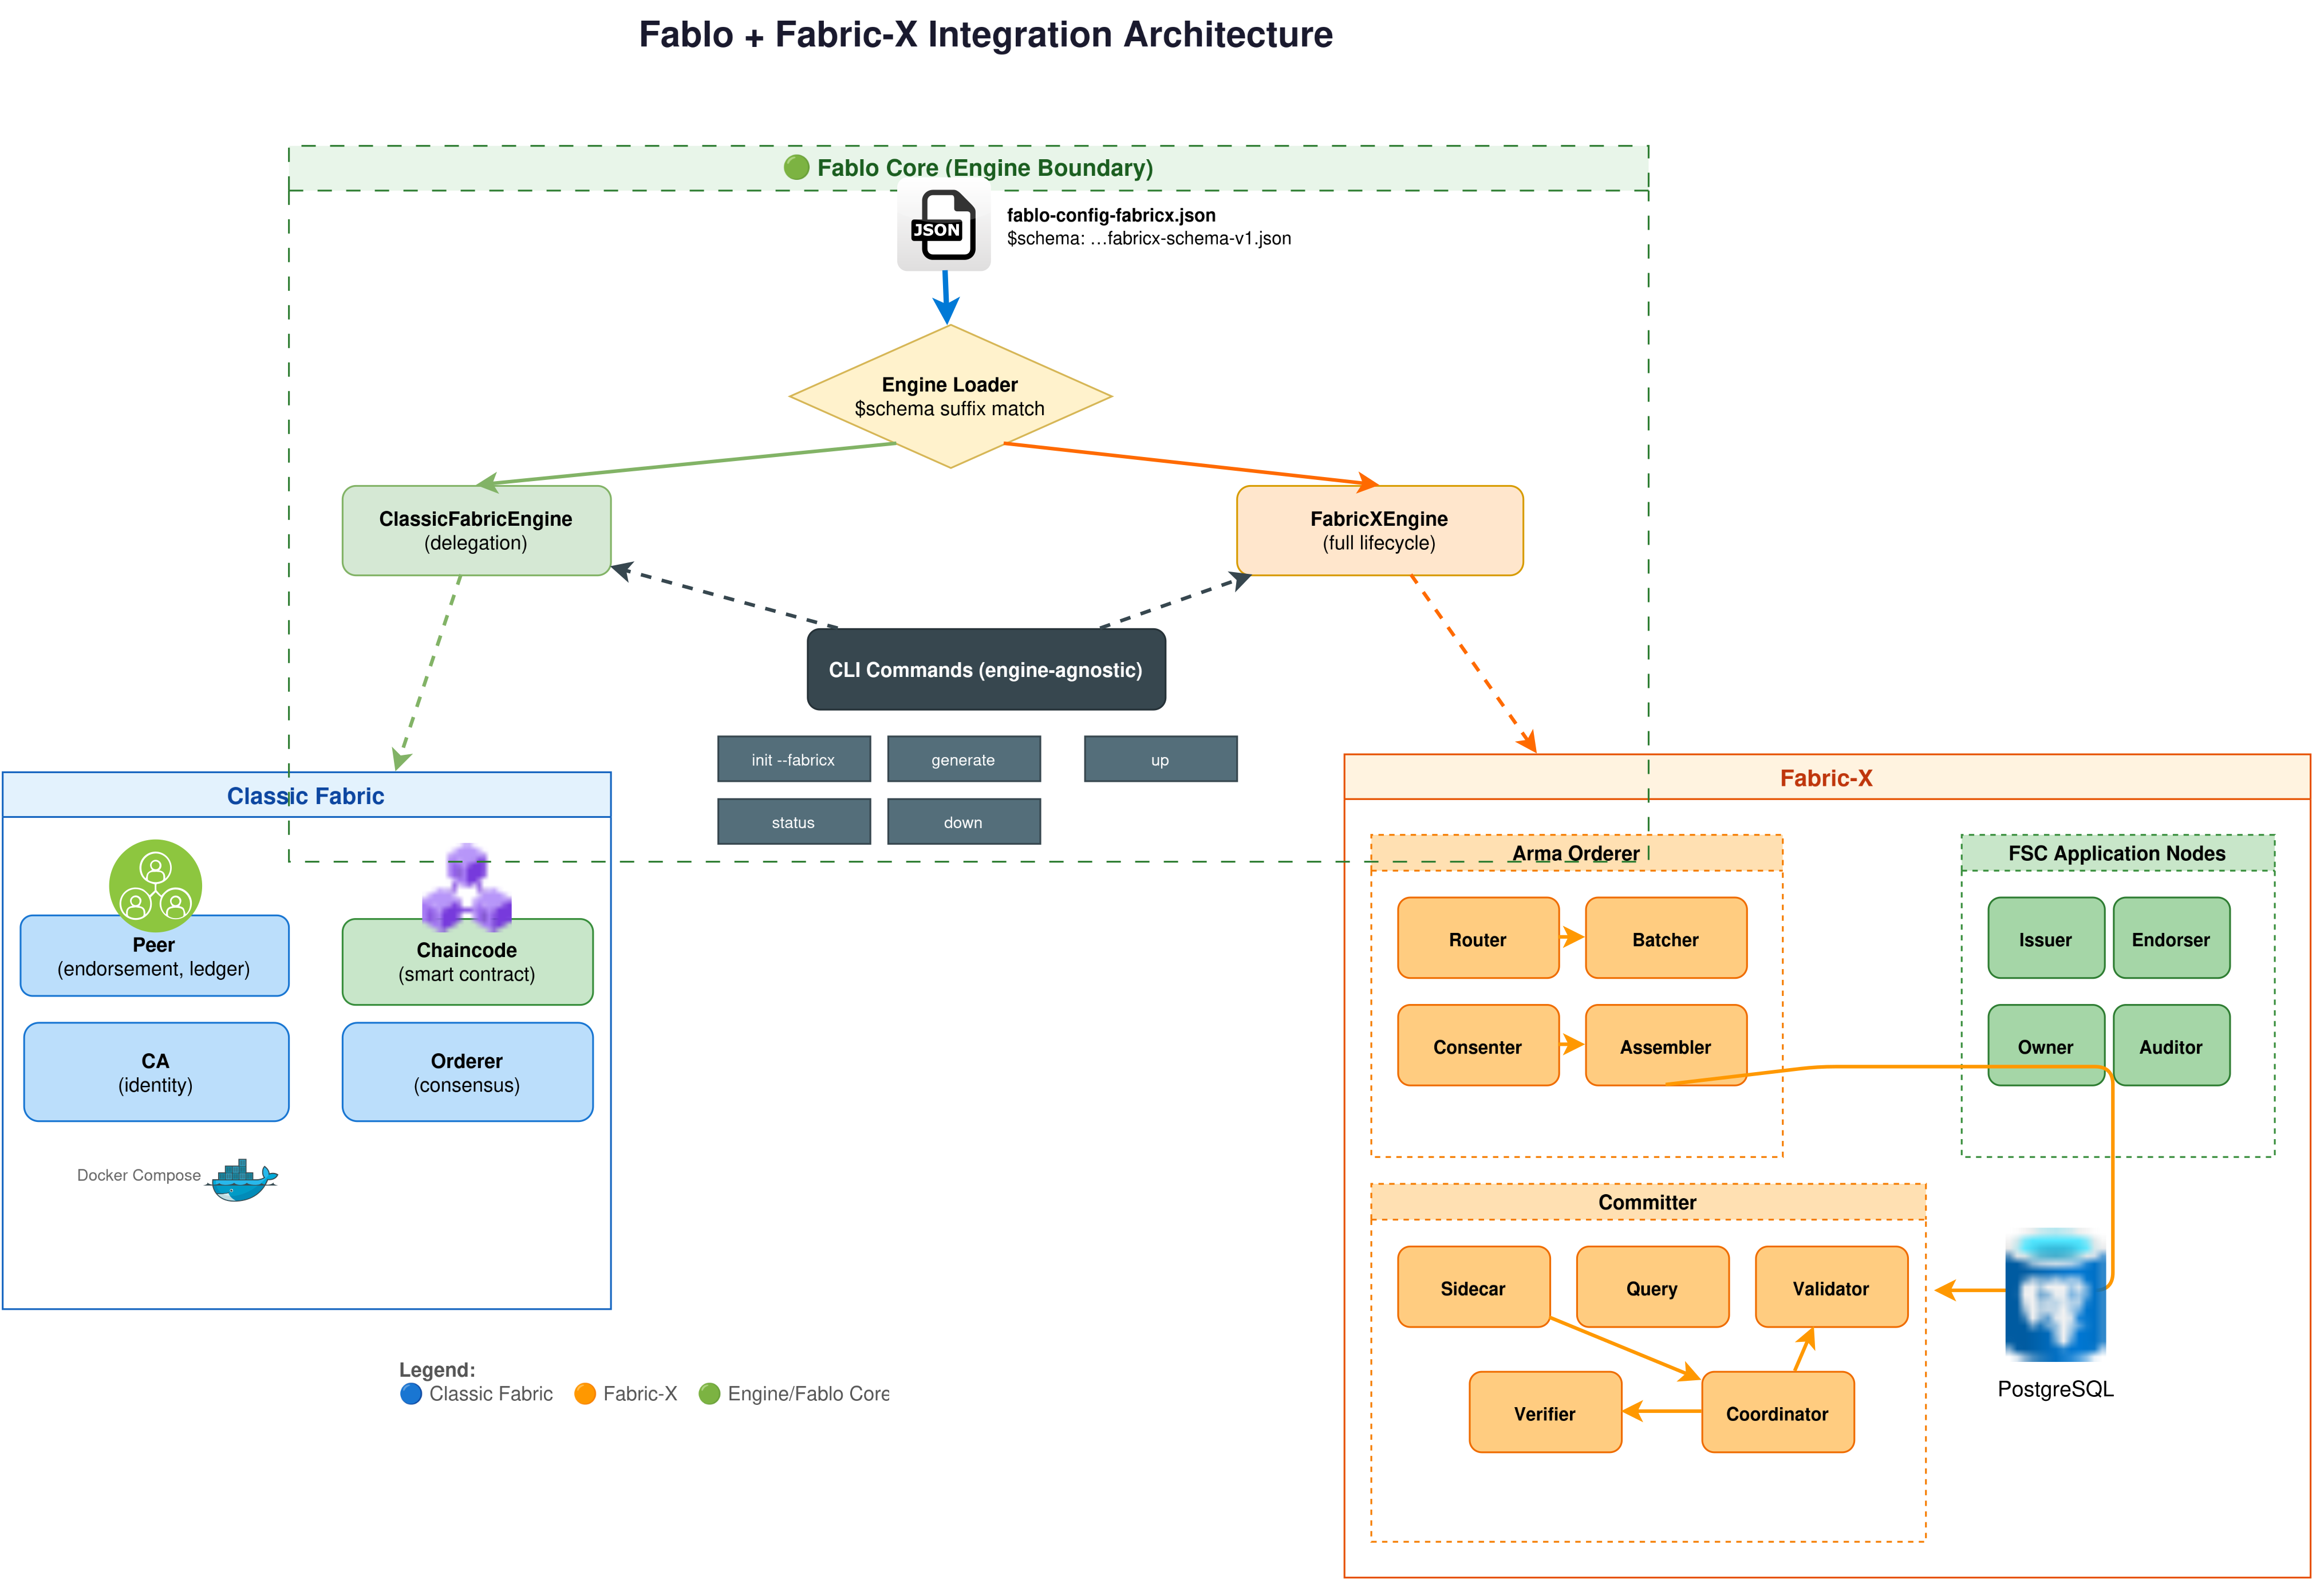
\includegraphics[width=\textwidth]{Fabric_fabricx_integration_architecture.png}
\caption{Fablo and Fabric-X integration architecture}
\label{fig:fablo-fabricx-architecture}
\end{figure}

\subsection{The Config Model: \texttt{extendFabricXConfig()}}

The natural analogue to classic Fablo's \texttt{extendConfig()} is a dedicated \texttt{extendFabricXConfig()} pass. The raw Fabric-X config should remain compact and intent-focused. The extension pass computes the derived information that templates need so that the EJS layer stays simple and mostly branch-free. This is exactly how classic Fablo works today: the user does not hand-author internal addresses, image tags, or every port binding. The generator computes those once and then renders deterministic output.

This is also where I directly apply the mentor feedback on schema design. I agree that Fabric-X should have its own \texttt{\$schema} rather than sharing the classic Fabric schema behind a global flag. Fabric-X differs structurally enough from classic Fabric that a shared schema would either become bloated with conditional rules or become too weak to validate meaningfully. A dedicated schema keeps validation cleaner, keeps the engine boundary explicit, and makes future schema evolution easier to reason about.

There are three categories of derived state that matter most. First is image resolution. Classic Fablo uses \texttt{extendGlobal()} to map one \texttt{fabricVersion} to a tested set of Fabric images. Fabric-X cannot yet do that safely because the relevant components evolve on separate cadences: the orderer, committer, tools image, and database all have independent versioning. The PoC therefore keeps images explicit. The Full Technical Implementation should still preserve the same abstraction boundary by letting \texttt{extendFabricXConfig()} map a future \texttt{fabricxVersion} profile to a tested image set, while still supporting explicit overrides when upstream release cadences drift.

Second is port allocation. Classic Fablo derives peer and orderer port ranges by walking org and instance indexes. Fabric-X needs the same determinism, but across a larger service surface. Even a single local network may need ports for router, batcher, consenter, assembler, sidecar, query service, validator-committer, verifier, coordinator, database, and multiple FSC node APIs and P2P listeners. The important point is not any one number. It is that users should declare topology, not manually wire every host-side port relationship. \texttt{extendFabricXConfig()} should own that translation.

Third, and most important, is inter-service wiring. In the decomposed architecture, the orderer roles are not independent containers that can be rendered in isolation. Routers need batcher shard endpoints. Assemblers need batcher and consenter addresses. The committer coordinator needs verifier and validator-committer addresses. Sidecars need assembler addresses. FSC nodes need sidecar, query service, and eventually notification service endpoints. Those relationships are exactly the kind of glue logic that should be derived once inside the extension pass rather than repeated in templates or exposed as user burden.

There is also a user-experience concern I want to address explicitly. Requiring the user to pass the config path and target directory on every command is workable for a proof of concept, but it is not the right long-term Fablo experience. As part of the local UX hardening phase, I plan to support a cleaner default flow through config autodiscovery or a local state file so that repeated commands do not require repetitive path arguments.

\begin{tcolorbox}[colback=gray!5!white, colframe=gray!50!black,
  title=Planned Fabric-X extended config contract,
  fonttitle=\bfseries, arc=4pt]
\begin{lstlisting}[language=typescript, basicstyle=\ttfamily\small]
export interface FabricXExtendedConfig {
  topology: "xdev" | "decomposed";
  images: {
    orderer: string;
    committer: string;
    tools: string;
    postgres: string;
  };
  channel: {
    name: string;
    profile: string;
    namespace: string;
    policy: string;
  };
  ordererOrgs: Array<{
    name: string;
    domain: string;
    groupId: number;
    router: { address: string; rpcPort: number; metricsPort: number; };
    batcher: { address: string; rpcPort: number; metricsPort: number; shardId: number; };
    consensus: { address: string; rpcPort: number; metricsPort: number; };
    assembler: { address: string; rpcPort: number; metricsPort: number; };
  }>;
  committer: {
    database: { type: "postgres" | "yugabyte"; host: string; port: number; };
    validator: { address: string; rpcPort: number; metricsPort: number; };
    verifier: { address: string; rpcPort: number; metricsPort: number; };
    coordinator: { address: string; rpcPort: number; metricsPort: number; };
    sidecar: { address: string; rpcPort: number; metricsPort: number; };
    queryService: { address: string; rpcPort: number; metricsPort: number; };
  };
  nodes: Array<{
    id: string;
    role: "issuer" | "endorser" | "owner";
    organization: string;
    apiPort: number;
    p2pPort: number;
    sidecarAddress: string;
    queryAddress: string;
  }>;
}
\end{lstlisting}
\end{tcolorbox}

The corresponding v2 schema should make the decomposed topology explicit rather than trying to hide it behind overloaded PoC fields:

\begin{tcolorbox}[colback=gray!5!white, colframe=gray!50!black,
  title=Planned v2 Fabric-X config (illustrative),
  fonttitle=\bfseries, arc=4pt]
\begin{lstlisting}[language=json, basicstyle=\ttfamily\footnotesize]
{
  "$schema": "https://fablo.io/schemas/fabricx-schema-v2.json",
  "global": { "fabricVersion": "x", "tls": false },
  "fabricx": {
    "topology": "decomposed",
    "channel": {
      "name": "arma",
      "namespace": "token_namespace",
      "policy": "AND('Org1MSP.member')"
    },
    "ordererOrgs": [
      {
        "name": "OrdererOrg1",
        "domain": "ordererorg1.example.com",
        "groupId": 1,
        "router": { "rpcPort": 7050, "metricsPort": 7060 },
        "consensus": { "rpcPort": 7051, "metricsPort": 7061 },
        "assembler": { "rpcPort": 7052, "metricsPort": 7062 },
        "batcher": { "rpcPort": 7053, "metricsPort": 7063, "shardId": 1 }
      }
    ],
    "committer": {
      "database": { "type": "postgres", "port": 5150 },
      "validator": { "rpcPort": 5100, "metricsPort": 5200 },
      "verifier": { "rpcPort": 5110, "metricsPort": 5210 },
      "coordinator": { "rpcPort": 5120, "metricsPort": 5220 },
      "sidecar": { "rpcPort": 5130, "metricsPort": 5230 },
      "queryService": { "rpcPort": 5140, "metricsPort": 5240 }
    },
    "nodes": [
      { "id": "issuer", "role": "issuer", "organization": "Org1" },
      { "id": "endorser1", "role": "endorser", "organization": "Org1" },
      { "id": "owner1", "role": "owner", "organization": "Org1" }
    ]
  }
}
\end{lstlisting}
\end{tcolorbox}

This is the critical architectural point: the engine interface does not need to change for any of this. The work is concentrated in the Fabric-X extension pass and the templates it feeds, exactly as classic Fablo concentrates classic-Fabric topology expansion inside \texttt{extendConfig()} and the render pipeline.

\subsection{The Template Set}

The template strategy for full Fabric-X support should mirror the structure that already makes classic Fablo maintainable: one master Compose template, one service-config template per role, and a clear split between derived config and rendered artifacts. The important point is not the original template language used elsewhere, but that the final Fablo templates should follow the same role-by-role structure for router, batcher, consensus, assembler, validator, verifier, coordinator, sidecar, and query service. Those variables then map cleanly from \texttt{extendFabricXConfig()} into EJS.

\begin{tcolorbox}[colback=gray!5!white, colframe=gray!50!black,
  title=Planned Fabric-X template tree,
  fonttitle=\bfseries, arc=4pt]
\begin{lstlisting}[language={}, basicstyle=\ttfamily\footnotesize]
src/engines/fabricx/templates/
├── docker-compose.fabricx.yaml.ejs
├── orderer/
│   ├── config-router.yaml.ejs
│   ├── config-batcher.yaml.ejs
│   ├── config-consensus.yaml.ejs
│   └── config-assembler.yaml.ejs
├── committer/
│   ├── config-validator.yaml.ejs
│   ├── config-verifier.yaml.ejs
│   ├── config-coordinator.yaml.ejs
│   ├── config-sidecar.yaml.ejs
│   └── config-query-service.yaml.ejs
├── fsc/
│   ├── core.yaml.ejs
│   └── routing-config.yaml.ejs
└── scripts/
    ├── bootstrap.sh.ejs
    └── reset.sh.ejs
\end{lstlisting}
\end{tcolorbox}

The master compose template should then iterate the same way classic Fablo iterates orgs and peers today. Instead of walking \texttt{orgs[].peers[]}, it walks \texttt{ordererOrgs[]} and emits four orderer-role service blocks for each group, then emits the committer-family services and any application nodes declared by the user. In other words, the implementation pattern remains recognizably Fablo even though the runtime model is different.

\begin{tcolorbox}[colback=gray!5!white, colframe=gray!50!black,
  title=Master Fabric-X compose iteration (illustrative),
  fonttitle=\bfseries, arc=4pt]
\begin{lstlisting}[language=ejs, basicstyle=\ttfamily\footnotesize]
services:
<% ordererOrgs.forEach((org) => { %>
  <%- include("orderer/router-service", { org }) %>
  <%- include("orderer/batcher-service", { org }) %>
  <%- include("orderer/consensus-service", { org }) %>
  <%- include("orderer/assembler-service", { org }) %>
<% }) %>
  <%- include("committer/database-service", { committer }) %>
  <%- include("committer/validator-service", { committer }) %>
  <%- include("committer/verifier-service", { committer }) %>
  <%- include("committer/coordinator-service", { committer }) %>
  <%- include("committer/sidecar-service", { committer }) %>
  <%- include("committer/query-service", { committer }) %>
\end{lstlisting}
\end{tcolorbox}

The startup order also has to be rendered deliberately. The same dependency chain appears consistently across the existing deployment patterns: the database must be healthy first, then the orderer subsystem, then the committer services that consume it, and finally the FSC nodes that depend on sidecar and query endpoints. In Compose terms, the important order is database $\rightarrow$ orderer roles $\rightarrow$ validator/verifier/coordinator $\rightarrow$ sidecar/query service $\rightarrow$ FSC application nodes. That is where existing deployment patterns are useful as correctness references for environment variables, health checks, and mounts.

\subsection{Crypto Pipeline}

The PoC already moved one important step in the right direction by generating crypto material and a genesis block through Dockerized tooling instead of expecting manual host setup. Full Fabric-X integration has to carry that idea further until all local bootstrap artifacts are produced automatically. The remaining gap is the richer identity flow used in current local Fabric-X bootstraps: starting a Fabric CA, enrolling a CA admin, registering and enrolling owner identities, issuing TLS identities for FSC nodes, and then generating token parameters.

That leads naturally to a three-stage pipeline. Stage one generates the classic Fabric MSP and TLS tree required for orderer compatibility and genesis construction. Stage two uses Fabric CA enrollment to issue FSC node certificates and owner wallets. Stage three runs \texttt{tokengen} to produce the namespace parameters consumed by token-enabled application nodes. Each stage should be executed through short-lived Docker containers so that the user still only needs Docker and Node.js, which preserves the central Fablo promise.

\begin{tcolorbox}[colback=gray!5!white, colframe=gray!50!black,
  title=Planned crypto generation contract,
  fonttitle=\bfseries, arc=4pt]
\begin{lstlisting}[language=typescript, basicstyle=\ttfamily\small]
export interface FabricXCryptoOutputs {
  genesisBlockPath: string;
  ordererMspDirs: Record<string, string>;
  nodeMspDirs: Record<string, string>;
  nodeTlsDirs: Record<string, string>;
  ownerWalletDirs: Record<string, string>;
  namespaceParametersDir: string;
}

export interface FabricXCryptoGenerator {
  generate(config: FabricXExtendedConfig, targetDir: string): Promise<FabricXCryptoOutputs>;
  validate(outputs: FabricXCryptoOutputs): Promise<void>;
}
\end{lstlisting}
\end{tcolorbox}

The advantage of expressing this as an internal generator contract is that it keeps the complexity contained. The command layer still sees only \texttt{generate()}. The Fabric-X engine is free to evolve from today's simpler genesis-and-MSP bootstrap into a fuller CA- and token-aware pipeline without destabilizing classic Fabric code paths.

\subsection{CCaaS and Contract Integration}

A full Fabric-X path that only boots infrastructure is incomplete. Classic Fablo's practical value comes from describing not only the network, but also the contracts attached to it. Fabric-X needs the same capability in its own terms. The relevant analogue is a \texttt{chaincodes} section that tells the engine which contract services should be started, where their source lives, and which endorser-side endpoint should consume them. This aligns with both the existing classic Fablo mental model and the Fabric-X sample topology, where the endorser role is application-relevant rather than incidental.

\begin{tcolorbox}[colback=gray!5!white, colframe=gray!50!black,
  title=Planned Fabric-X contract config,
  fonttitle=\bfseries, arc=4pt]
\begin{lstlisting}[language=json, basicstyle=\ttfamily\footnotesize]
{
  "fabricx": {
    "chaincodes": [
      {
        "name": "tokencc",
        "lang": "ccaas",
        "directory": "./chaincodes/tokencc",
        "endpoint": "tokencc:9999",
        "endorser": "endorser1"
      }
    ]
  }
}
\end{lstlisting}
\end{tcolorbox}

Once that exists, Fablo can generate the corresponding CCaaS service blocks, volumes, and helper commands in the same way it already does for classic Fabric. This matters because the target user experience is not ``a network that technically starts.'' It is ``a network a developer can actually use to run and test a contract.''

\subsection{Lifecycle Hardening}

The bundled PoC path is intentionally lightweight, but the full implementation has to take lifecycle management more seriously. In classic Fablo, a reset is mostly about stopping containers and clearing generated network state. In Fabric-X, there is a larger state surface: generated per-role service configs, generated crypto material, namespace artifacts, database state, and the Fabric-X engine state file that records what was rendered. A plain \texttt{docker compose down} is therefore not a sufficient definition of reset.

\begin{tcolorbox}[colback=gray!5!white, colframe=gray!50!black,
  title=Planned Fabric-X reset flow,
  fonttitle=\bfseries, arc=4pt]
\begin{lstlisting}[language=typescript, basicstyle=\ttfamily\small]
async reset(targetDir?: string): Promise<void> {
  const dir = resolveTargetDir(targetDir);
  const composeFile = path.join(dir, "docker-compose.fabricx.yaml");

  if (await fs.pathExists(composeFile)) {
    await runDockerCompose(dir, ["down", "-v", "--remove-orphans"]);
  }

  await fs.remove(path.join(dir, "services"));
  await fs.remove(path.join(dir, "input"));
  await fs.remove(path.join(dir, "fxconfig"));
  await fs.remove(path.join(dir, "fabricx-engine-state.json"));
}
\end{lstlisting}
\end{tcolorbox}

The same hardening logic applies to helper commands. In classic Fablo, channel helpers are part of the user contract because channels are a first-class lifecycle concern. In Fabric-X, the equivalent surface is \texttt{fxconfig}. Namespace creation, namespace listing, and later namespace update operations should be exposed as first-class helper flows once the decomposed engine is stable enough. That keeps the conceptual model coherent: classic Fabric gets channel-aware tooling; Fabric-X gets namespace-aware tooling.

\subsection{Testing Strategy}

The test strategy should grow from the exact style Fablo already uses rather than inventing a parallel harness. The current Fabric-X happy-path test already proves the bundled topology can be initialized, generated, started, queried, and torn down. The Full Technical Implementation plan is to extend that into a small but meaningful matrix of scenarios that exercise the engine at the right seams:
\begin{itemize}[leftmargin=*]
  \item generation-only validation: schema accepted, artifacts rendered, config files present
  \item happy-path \texttt{xdev} lifecycle: init $\rightarrow$ generate $\rightarrow$ up $\rightarrow$ namespace visible $\rightarrow$ status $\rightarrow$ down
  \item missing-artifact failure: clear error when a required generated file is absent or corrupt
  \item config validation failure: invalid topology rejected before generation begins
  \item decomposed topology bootstrap: one minimal decomposed network starts and reaches committer and query readiness
\end{itemize}

All of these tests should follow the existing \texttt{test-01-v3-simple.sh} discipline: create a temp workspace, build, run one focused scenario, assert on concrete artifacts and service health, and clean up. That matters because the most valuable thing Fablo can offer Fabric-X is not just code generation. It is a predictable, reviewable developer workflow that maintainers can trust not to regress silently.

\subsection{Documentation Deliverables}

The project description is not only asking for working code. It is also asking for a contribution that other users and maintainers can understand, extend, and review without reconstructing the design from commit history. For that reason, documentation is a first-class deliverable rather than cleanup work deferred to the end. The documentation plan has four concrete outputs.

First, I will maintain a user-facing \texttt{FABRICX.md} guide in the Fablo repository. This document will explain the Fabric-X config shape, the supported local workflow, the meaning of the generated target directory, the expected Docker prerequisites, and the lifecycle commands required to generate, start, inspect, and tear down a Fabric-X network. For the PoC, it will document the bundled \texttt{xdev} path exactly as implemented. As the decomposed topology lands, the same guide will expand to explain the richer schema and service model instead of forcing users to read source code or proposal text.

Second, I will write architecture decision records for the main design choices that shape the implementation. At minimum, these records should capture the engine split, schema-first engine detection via \texttt{\$schema}, and the decision to start with the bundled \texttt{xdev} topology instead of claiming decomposed production parity on day one. These ADRs matter because they preserve the reasoning behind the implementation boundary. Future contributors should be able to see not just what the code does, but why the project chose a pluggable engine seam rather than a wrapper or a hard fork of the classic pipeline.

Third, I will add a contributor guide that explains how to add a third engine. This is the logical follow-through of the engine architecture. If the interface is a real extension seam, the repository should document how a new engine declares its schema, plugs into engine selection, implements lifecycle methods, contributes templates, and adds e2e tests without disturbing existing engines. This guide will help reviewers confirm that the engine abstraction is general rather than accidental.

Finally, I will add inline code documentation on all public interfaces introduced by the work. That includes the engine contract, engine loader, shared helper utilities, and the public Fabric-X-specific types that future maintainers will extend. This level of documentation is especially important because the project crosses multiple domains: Oclif command routing, JSON schema validation, template rendering, Docker orchestration, and Fabric-X bootstrap logic. Good inline documentation reduces the risk that the Fabric-X path becomes understandable only to the original author.

\begin{tcolorbox}[colback=gray!5!white, colframe=gray!50!black,
  title=Documentation deliverables,
  fonttitle=\bfseries, arc=4pt]
\begin{itemize}[leftmargin=*]
  \item \texttt{FABRICX.md}: user-facing setup and lifecycle guide
  \item Architecture decision records: engine split, schema-first detection, bundled \texttt{xdev} scope choice
  \item Contributor guide: how to add a third engine cleanly
  \item Inline code documentation on all public interfaces and extension points
\end{itemize}
\end{tcolorbox}

\section{Known Limitations and How They Will Be Resolved}

\begin{tcolorbox}[colback=yellow!5!white, colframe=yellow!60!black,
  title=Known PoC Limitations (all isolated inside the new engine architecture),
  fonttitle=\bfseries, arc=4pt]
\begin{itemize}[leftmargin=*]
\item \textbf{Bundled \texttt{xdev} topology only.} The current engine targets the FSC-style test-node path, not the full decomposed deployment with separate router, batcher, consenter, assembler, validator, verifier, coordinator, sidecar, and query containers.
\item \textbf{Single-org local bootstrap.} The verified path is a single-organization local network. Multi-orderer-group and multi-organization policy topologies remain future work.
\item \textbf{TLS disabled in the current happy path.} The validated MVP follows the current FSC local-default pattern with \texttt{tls=false}. Full TLS and mTLS support for orderer, committer, and helper tooling are not yet hardened.
\item \textbf{PostgreSQL only.} Yugabyte-backed local generation is not implemented yet.
\item \textbf{No full CA/Idemix/\texttt{tokengen} pipeline yet.} The MVP now automates MSP and genesis generation with Dockerized tooling and bootstraps namespaces through \texttt{fxconfig}, but the richer Fabric-CA-based owner and FSC-node enrollment flow shown in \texttt{gen\_crypto.sh} is still part of the beyond-MVP work.
\item \textbf{Docker Compose only.} Kubernetes and OpenShift manifests are not generated.
\end{itemize}
All of these limitations are confined to \texttt{src/engines/fabricx/} and cannot affect classic Fabric functionality.
\end{tcolorbox}

The important point is not that the PoC has limitations; all credible proofs of concept do. The important point is that each limitation is already isolated and explained. The engine split ensures that classic Fabric behavior remains unaffected. I have also defined the replacement path for each shortcut directly in this proposal, which keeps the mentorship plan reviewable and lowers the risk of architectural drift.

\section{Pre-Application Research}

\begin{tcolorbox}[colback=green!5!white, colframe=green!60!black,
  title=Pre-Application Research Completed, fonttitle=\bfseries, arc=4pt]
Before writing this proposal, I completed research that was specific enough to de-risk the design rather than just survey the codebase:
\begin{itemize}[leftmargin=*]
  \item Reading \texttt{fablo/src/engines/engine.ts} confirmed that the clean extension seam is a small lifecycle-shaped interface with \texttt{validate}, \texttt{generate}, \texttt{up}, \texttt{down}, and \texttt{status}, which is why I treated Fabric-X as a separate engine instead of adding more branching to the classic path.
  \item Reading \texttt{fabric-smart-client/integration/nwo/fabricx/extensions/scv2/container.go} confirmed the exact bundled test-node container contract: the crypto tree must be mounted at \texttt{/root/artifacts/crypto}, the config block must be mounted at \texttt{/root/artifacts/config-block.pb.bin}, Linux requires \texttt{host.docker.internal:host-gateway}, and sidecar, query, and ordering ports are all bound explicitly. This was the key source for fixing the broken container mounts in the original Fablo Fabric-X draft.
  \item Reading \texttt{fabric-smart-client/integration/nwo/fabricx/extensions/v3/test\_utils.go} confirmed the actual bundled local startup command, \texttt{run db orderer committer --insecure}, and the current sidecar environment-variable pattern. That let me align the generated Compose file with the working FSC integration instead of guessing the container entrypoint.
  \item Reading \texttt{fabric-smart-client/integration/nwo/fabricx/fxconfig/namespace.go} clarified the namespace bootstrap contract. In particular, it showed the exact \texttt{FXCONFIG\_*} environment variables required for MSP identity, orderer access, notifications, and query access, which is why the PoC uses generated environment wiring instead of ad hoc shell commands.
  \item Reading \texttt{fabric-x-ansible-collection/examples/inventory/local/fabric-x.yaml} together with the orderer and committer role templates confirmed that the full topology is not a single peer-and-orderer variation: the orderer is split into router, batcher, consensus, and assembler, while the committer stack is split into validator, verifier, coordinator, sidecar, query service, and database. That finding is the reason the proposal treats the bundled path as a PoC and the decomposed path as the final implementation target.
  \item Reading \texttt{fabric-x-samples/tokens/scripts/gen\_crypto.sh} showed that the richer local crypto flow includes Fabric CA startup, owner enrollment, FSC node TLS enrollment, and token-parameter generation. That is why I describe the current automated MSP and genesis generation honestly as a partial bootstrap pipeline rather than as the complete Fabric-X crypto story.
  \item Running the local flow exposed a concrete runtime issue in namespace bootstrap: \texttt{fxconfig namespace create --endorse --submit --wait} did not give a reliable completion signal in the current bundled setup, so I verified that submitting first and then polling visible namespace state through \texttt{fxconfig namespace list} is the more stable supported PoC path.
  \item Running the generated bootstrap also exposed an orderer configuration issue: when the generated config advertised separate broadcast and deliver endpoints for the same bundled orderer path, the sidecar became unstable. I fixed this by aligning the generated orderer endpoint shape with the current Fabric-X local expectations described in the research and validation notes.
\end{itemize}
\end{tcolorbox}

This pre-application work is important because it changes the proposal from speculative to evidence-based. The working PoC is not presented as final software, but it is strong proof that the architectural direction is sound and that the candidate has already navigated the difficult parts of the codebase.
\section{Risk Register}

\begin{table}[h]
\centering
\begin{tabularx}{\textwidth}{|p{3cm}|X|p{2cm}|}
\hline
\textbf{Risk} & \textbf{Mitigation strategy} & \textbf{Probability} \\
\hline
Fabric-X API surfaces change before stable release &
Keep version-sensitive behavior isolated inside
the Fabric-X engine; pin images explicitly
in the schema; the \texttt{\$schema} versioning
strategy means a breaking upstream change requires
a new schema version rather than patching live code. &
Medium \\
\hline
Crypto generation for FSC nodes is underdocumented &
Treat the current local bootstrap flow as the working
specification; implement the pipeline in stages with
a validated fallback to externally supplied material
at each stage boundary so the MVP is never blocked
by an incomplete later stage. &
High \\
\hline
Mentor review cycles slow down PR merges &
Submit small, reviewable PRs aligned to phase
boundaries rather than large feature branches;
use the engine isolation to keep each PR
self-contained and non-breaking for classic Fabric. &
Medium \\
\hline
xdev topology diverges further from decomposed
production model before Phase 3 begins &
The schema explicitly carries a \texttt{topology}
field; xdev and decomposed are separate code paths
from day one, so upstream changes to the bundled
image do not block decomposed work and vice versa. &
Low \\
\hline
Stretch goals displace core hardening work &
Stretch work begins only after the core deliverables
checklist is fully merged; the engine boundary and
the known limitations list are the explicit
scope gate. &
Medium \\
\hline
\end{tabularx}
\caption{Risk register with mitigation strategies}
\label{tab:risks}
\end{table}

Every risk above is tied to something concretely observable:
version drift between components, crypto complexity in the
current local bootstrap flow, and the normal review latency
of upstream open source work. Naming real risks makes them tractable.

% ─────────────────────────────────────────────
\section{Success Metrics}
% ─────────────────────────────────────────────

\subsection*{Already Verified Foundations}

These items are already demonstrated by the pre-application PoC and reduce the risk of the project:
\begin{itemize}[leftmargin=2em]
  \item schema-based Fabric-X engine selection is viable
  \item a simple local Fabric-X bootstrap flow can be driven through Fablo-style lifecycle commands
  \item automated validation for the supported happy path is achievable
\end{itemize}

\subsection*{Core Deliverables}

The following items are the minimum acceptable outcome for this mentorship. These are the deliverables I am proposing for the funded work, and all must be merged and independently reproducible before the final evaluation.

\begin{tcolorbox}[colback=green!5!white, colframe=green!60!black,
  title=Core Deliverables, fonttitle=\bfseries, arc=4pt]
\begin{itemize}[leftmargin=2em]
  \item[\checkmark] A design proposal and architectural recommendation accepted upstream
  \item[\checkmark] A supported Fabric-X config and workflow for a simple local network through Fablo
  \item[\checkmark] A local bootstrap flow with working lifecycle commands and namespace setup
  \item[\checkmark] Example configurations and a sample workflow that others can reproduce
  \item[\checkmark] Automated validation for the supported Fabric-X scenario
  \item[\checkmark] \texttt{FABRICX.md}, architecture decision records, and a contributor guide for extending the engine model
  \item[\checkmark] A documented path from the supported bundled local workflow toward richer decomposed topologies
\end{itemize}
\end{tcolorbox}

\subsection*{Stretch Goals}

The following items begin only after every core deliverable
above is merged. They are not commitments; they are the
natural next layer of work if schedule permits.

\begin{itemize}[leftmargin=2em]
  \item Dynamic crypto pipeline: Fabric CA enrollment and
        \texttt{tokengen} replacing copied sample material
  \item Decomposed topology: separate router, batcher,
        consenter, assembler, and committer-family containers
        generated from a \texttt{topology: decomposed} config
  \item Multi-org endorsement policy support with
        multi-organization crypto generation
  \item CI integration example showing a Fabric-X network
        bootstrapped inside a GitHub Actions workflow
\end{itemize}
